\documentclass[10pt]{article}
\usepackage[utf8]{inputenc}
\usepackage[T1]{fontenc}
\usepackage{amsmath}
\usepackage{amsfonts}
\usepackage{amssymb}
\usepackage[version=4]{mhchem}
\usepackage{stmaryrd}
\usepackage{bbold}
\usepackage{graphicx}
\usepackage[export]{adjustbox}
\graphicspath{ {./images/} }

\begin{document}
\section*{Lecture hours 24-26}
\section*{Definitions and Theorems}
Definition ( Transpose of a matrix Matrix).\\
The transpose of a matrix $A$ is $A^{T}$, and it has columns the rows of A (same order).

Definition ( Perpendicular complement).\\
Let $V$ be a subspace of $\mathbb{R}^{n}$, then $W$ is called the "perpendicular complement" of $V$ and denoted $V^{\perp}$ (pronounced "V perp", symbol $\perp$ is a superscript ) if $W$ contains all vector in $\mathbb{R}^{n}$ that are perpendicular to all vectors in $V$.

Definition (Fundamental subspaces of linear algebra).\\
For any m by n matrix $A$ we have\\
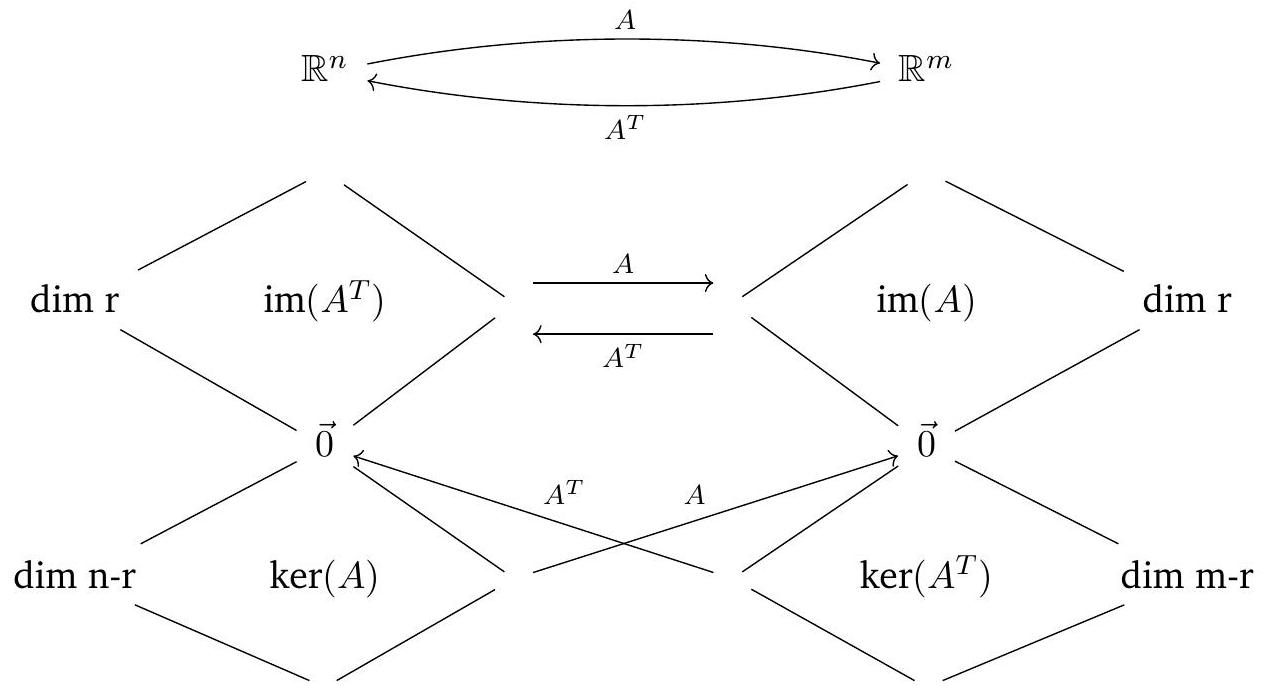
\includegraphics[max width=\textwidth, center]{2024_12_26_f858c68a27e2c0f87aabg-1}

$$
(\operatorname{ker} A)^{\perp}=\operatorname{im}\left(A^{T}\right), \quad(\operatorname{im} A)^{\perp}=\operatorname{ker}\left(A^{T}\right)
$$

Problem 43 (Fundamental subspaces of linear algebra). Consider the matrix

$$
A=\left[\begin{array}{cc}
2 & 1 \\
-1 & 0 \\
0 & 0
\end{array}\right]
$$

Find $\operatorname{ker}(A), \operatorname{im}(A), \operatorname{ker}\left(A^{T}\right)$, and $\operatorname{im}\left(A^{T}\right)$. For each of these subspaces, determine the value of $n$ for which they are a subspace of $\mathbb{R}^{n}$.

Problem 44 (Transpose of a matrix). Let $A$ be an invertible $n \times n$ matrix.\\
a) Explain why $A^{T}$ is invertible.\\
b) Explain why $\left(A^{T}\right)^{-1}=\left(A^{-1}\right)^{T}$. (Hint: $I^{T}=I$.)

Problem 45 (Least squares - Normal Equations). You are given data points $(x, y)=$ $(1,1),(2,3),(-1,3)$. Use a least squares line of best fit to predict the $y$-value when $x=7$.


\end{document}